\documentclass{article}
\usepackage{graphicx} % Required for inserting images
\usepackage{amsmath}
\usepackage{float}
\usepackage{booktabs}
\usepackage{subcaption}
\usepackage{multirow}
\usepackage[inline]{enumitem}
\usepackage{pgfplots}
\pgfplotsset{compat=1.18}


\title{Combinatorial Decision Making and Optimization}
\author{Tomaž Cotič}
\date{September 2025}

\begin{document}

% \maketitle

\section{CP Model}

\subsection{Decision Variables}
The CP model relies on the following decision variables:

\begin{itemize}
    \item For each pair of teams $(i,j)$ we define $\text{\textbf{period}}_{i,j} \in P\}$ as the slot in which team $i$ plays against team $j,$ where $n$ is the number of teams that take part in the tournament.
    \item Similarly, for each pair of teams $(i,j)$ we define the variables $\text{\textbf{home}}_{i,j}\in \{0, 1\}$ in such a way that $\text{home}_{i,j}=1$ when $i$ plays against $j$ at home.
\end{itemize}

Moreover, using the previously described \emph{circle method}, all week assignments are precomputed and passed to the model in the variables $\text{\textbf{week}}_{i,j} \in W$, where $\text{week}_{i,j} = w$ means that $i$ plays against $j$ in week $w$.

\subsection{Objective Function}
As already described above, the objective function is defined as
\[
\max_{t \in T} \, |H_t - A_t|,
\]
where \(H_t\) is the number of home games of team \(t\), \(A_t\) is the number of away games of team \(t\), and \(T\) is the set of teams.

In the CP model, the number of games each team plays at home and away are stored in two arrays:
\[
\forall t \in T \quad \mathtt{home\_count[t]} \in \{1, \dots, n-1\}, 
\qquad
\mathtt{away\_count[t]} \in \{1, \dots, n-1\}.
\]
The imbalance for each team is stored in
\[
\mathtt{imbalance[t]} = \lvert \mathtt{home\_count[t]} - \mathtt{away\_count[t]} \rvert,
\qquad t \in T,
\]
and the optimization variable is taken as
\[
\max_{t \in T} \mathtt{imbalance[t]}.
\]

A final consideration regarding the objective function is that the CP models performed significantly better when switching from minimizing the sum of home–away imbalances to minimizing the maximum imbalance.

\subsection{Constraints}
The \emph{circle method} automatically satisfies two of the three compulsory constraints:
\begin{enumerate}
    \item Each team plays every other team exactly once.
    \item Each team plays exactly once every week.
\end{enumerate}

In this way, only two constraints had to be implemented to solve the problem in a valid way:

\textbf{Each team plays at most twice in the same period:}
\[
\forall\, t \in T,\; \forall\, p \in P:\quad 
\sum_{j \in T \setminus \{t\}} \chi_{\{\text{period}_{t,j} = p\}} \;\leq\; 2
\]
We implemented this constraint using the global constraint \texttt{count\_geq}, which yielded better results than both the intuitive formulation and the alternative global constraint \texttt{global\_cardinality}.

\textbf{Each period in each week contains exactly one match:}
\[
\forall\, w \in W,\;
\forall\, p \in P:\quad
\sum_{\substack{(i,j) \in M}}
\chi_{\{\,\text{week}_{i,j} = w \,\wedge\, \text{period}_{i,j} = p\,\}} = 1,
\]
where $M$ is the set of all the possible matches: \[
M \;=\; \bigl\{\,(i,j) \;:\; i,j \in T,\; i<j \,\bigr\}.
\]
We tried to tackle this constraint using the global constraint \texttt{alldifferent} but it weakened the performance on basically all instances, which is why we didn't implement this constraint using the available global one.

Additional constraints were required due to the way we defined the decision variables. Specifically, we allowed the slot variable to take the value $0$, even though it does not correspond to a valid slot in which teams can play. Furthermore, the slot matrix is symmetric, and the home team assignment also exhibits a particular structure by design:
\begin{itemize}
    \item $\forall\, t \in T:\quad \text{period}_{t,t} = 0$
    \item  $\forall\, i,j \in T,\, i \ne j:\;
\begin{aligned}
& \text{period}_{i,j} \ne 0,\\
& \text{period}_{i,j} = \text{period}_{j,i},\\
& \text{home}_{j,i} = 1 - \text{home}_{i,j}
\end{aligned}$
\end{itemize}

\subsubsection*{Symmetry Breaking Constraints}
We identified some symmetries in the problem that, if left unaddressed,  enlarged the search space explored by the solver. To reduce redundant exploration, we introduced symmetry-breaking constraints:

\textbf{SB1: Fixing the slots of the first team:}
\[
\forall\, t \in T:\quad \text{period}_{1,t} \le \text{period}_{1,t+1}
\]

This constraint ensures that the slots assigned to the first team are strictly increasing, effectively removing symmetries that arise from permuting slot orders. We implemented it using the MiniZinc global constraint $\mathtt{increasing}.$

\textbf{SB2: Team 1's home/away pattern is fixed:}
\[
\forall\, w \in W:\quad
\text{home}_{1,\, w+1} =
\begin{cases}
1, & 1 \le w \le \lfloor \tfrac{\text{num\_teams}}{2} \rfloor,\\[2mm]
0, & \lfloor \tfrac{\text{num\_teams}}{2} \rfloor + 1 \le w \le \text{num\_teams}-1
\end{cases}
\]

This constraint eliminates symmetries that come from flipping home-away status forcing the first team to play the first half of the season at home and the second away.

\textbf{SB3: Imbalance ordering:}  

\[
\forall\, t \in T:\quad \text{imbalance}_t \ge \text{imbalance}_{t+1}
\]

This last symmetry breaking constraint binds the imbalance array to be decreasing and was of course tested only on the optimization version of the problem.

\subsection{Validation}
The models were implemented in MiniZinc and coupled with a Python script that takes the input parameters, determines week assignments, and subsequently executes the corresponding MiniZinc model.

\subsubsection{Experimental design}
We experimented our models using \textbf{Gecode} and \textbf{Chuffed} with different search strategies. All experiments were conducted respecting the given timeout of $300\,\mathrm{s}$, with the solvers in their sequential version and using $42$ as \texttt{random\_seed} in order to obtain a deterministic behavior.

\subsubsection{Experimental Results}

First, we present the results for the optimization version of the problem, followed by the results for the decision version at the end of the section in Figure~\ref{fig:solver_strategies}. Our first objective was to evaluate the impact of the proposed symmetry-breaking constraints. As shown in Table~\ref{cp-opt-results}, the inclusion of symmetry breaking yields clear benefits for both Gecode and Chuffed. In particular, Chuffed was able to solve the case $n=16$ to optimality, which was not possible without symmetry breaking. Similarly, Gecode, when combined with symmetry breaking, successfully solved the case $n=14$ to optimality. Among the three symmetry-breaking strategies considered, the best performance was obtained using the first two, while the third did not lead to any improvement in optimization time.

Having established the advantages of symmetry breaking, we next investigated alternative search strategies to further enhance performance. All subsequent experiments were conducted with symmetry breaking enabled.

For Chuffed, we identified two promising strategies:
\begin{enumerate*}[label=(\roman*)]
\item \texttt{first\_fail} for variable selection combined with \texttt{indomain\_split} for value assignment. We observed that changing the value assignment strategy had little, to no impact on the results,
\item \texttt{random\_order} for variable selection paired with a restart strategy using \texttt{Luby$(50)$}.
\end{enumerate*}
Both strategies yielded similar outcomes and improved the quality of the solution for $n=18$, although the computational time required for smaller instances increased noticeably, as it nearly doubled compared to the default Chuffed's search.

For Gecode, we initially experimented with the \texttt{first\_fail} variable selection heuristic, but it did not yield any performance improvement; consequently, we chose to omit it from the report. Switching to the largest-domain heuristic with weighted degree, combined with random value assignment, led to a significant improvement. Using this approach, Gecode was able to solve instances up to $n=16$ optimally, although, similar to Chuffed, the time required to solve $n=14$ increased noticeably.

We also attempted to combine this strategy with restarts, specifically \texttt{Luby}, but the results weakened. This trend was consistent across several restart scales arbitrarily chosen within $[20,100]$.

Additionally, we evaluated the large neighborhood search (LNS) strategy; however, it provided no benefit regardless of the retainment percentage, as shown in Table~\ref{cp-opt-results}.

Overall, Chuffed consistently outperformed Gecode, producing better results across nearly all non-trivial instances, with the exception of some faster solutions that Gecode was able to find for $n=16$. 

\begin{table}[h!]
\centering
\resizebox{\textwidth}{!}{%
\begin{tabular}{c|cccc|ccccc}
\toprule
\multirow{2}{*}{\textbf{n}} & \multicolumn{4}{c|}{\textbf{Chuffed}} & \multicolumn{5}{c}{\textbf{Gecode}} \\
\cmidrule(lr){2-5} \cmidrule(lr){6-10}
 & Base & SB & ff+indomain\_split & random+luby(50) & Base & SB & dwd+random & dwd+r+luby(50) & dwd+r+rr \\
\midrule
6  & $1\|\mathbf{1}$ & $1\|\mathbf{1}$ & $1\|\mathbf{1}$ & $1\|\mathbf{1}$ & $1\|\mathbf{1}$ & $1\|\mathbf{1}$ & $1\|\mathbf{1}$ & $1\|\mathbf{1}$ & $1\|\mathbf{1}$ \\
8  & $1\|\mathbf{1}$ & $1\|\mathbf{1}$ & $1\|\mathbf{1}$ & $1\|\mathbf{1}$ & $1\|\mathbf{1}$ & $1\|\mathbf{1}$ & $1\|\mathbf{1}$ & $1\|\mathbf{1}$ & $1\|\mathbf{1}$ \\
10 & $1\|\mathbf{1}$ & $1\|\mathbf{1}$ & $1\|\mathbf{1}$ & $1\|\mathbf{1}$ & $1\|\mathbf{1}$ & $1\|\mathbf{1}$ & $1\|\mathbf{1}$ & $1\|\mathbf{1}$ & $1\|\mathbf{1}$ \\
12 & $2\|\mathbf{1}$ & $2\|\mathbf{1}$ & $1\|\mathbf{1}$ & $2\|\mathbf{1}$ & $2\|\mathbf{1}$ & $1\|\mathbf{1}$ & $1\|\mathbf{1}$ & $2\|\mathbf{1}$ & $1\|\mathbf{1}$ \\
14 & $20\|\mathbf{1}$ & $5\|\mathbf{1}$ & $19\|\mathbf{1}$ & $19\|\mathbf{1}$ & $300\|7$ & $2\|\mathbf{1}$ & $28\|\mathbf{1}$ & $22\|\mathbf{1}$ & $28\|\mathbf{1}$ \\
16 & $300\|5$ & $70\|\mathbf{1}$ & $144\|\mathbf{1}$ & $137\|\mathbf{1}$ & $\text{N/A}$ & $\text{N/A}$ & $18\|\mathbf{1}$ & $\text{N/A}$ & $17\|\mathbf{1}$ \\
18 & $\text{N/A}$ & $300\|13$ & $300\|7$ & $300\|7$ & $\text{N/A}$ & $\text{N/A}$ & $\text{N/A}$ & $\text{N/A}$ & $\text{N/A}$ \\
\bottomrule
\end{tabular}
}
\caption{Optimization version: runtime in seconds and found objective value for different combinations of models, solvers and search strategies.}
\label{cp-opt-results}
\end{table}

\begin{figure}[h!]
    \centering
    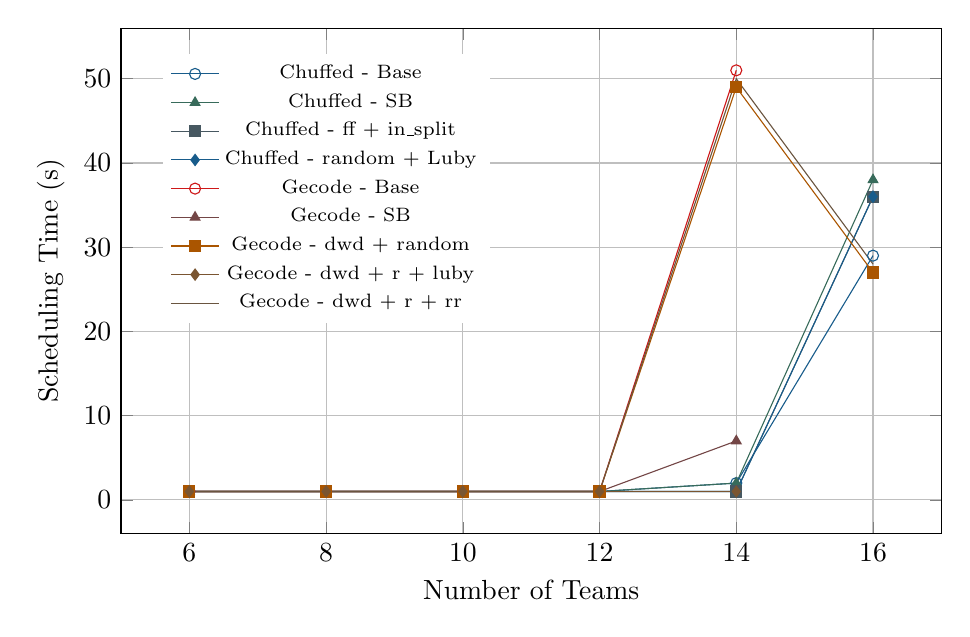
\begin{tikzpicture}
        \begin{axis}[
            xlabel={Number of Teams},
            ylabel={Scheduling Time (s)},
            grid=major,
            width=12cm,
            height=8cm,
            legend style={
                at={(0.05,0.95)},   % 5% from left, 95% from bottom
                anchor=north west,  % aligns the top-left of the legend to this             point
                font=\scriptsize,   % keeps it small
                draw=none            % optional: removes the box around legend
                },
        ]

        % Solver 1 (4 strategies) - blue shades
        \addplot[color={rgb:red,31;green,120;blue,180}, mark=o] coordinates {(6,1) (8,1) (10, 1) (12,1) (14,2) (16,29)};
        \addlegendentry{Chuffed - Base}

        \addplot[color={rgb:red,102;green,194;blue,165}, mark=triangle*] coordinates {(6,1) (8,1) (10, 1) (12,1) (14,2) (16,38)};
        \addlegendentry{Chuffed - SB}

        \addplot[color={rgb:red,166;green,206;blue,227}, mark=square*] coordinates {(6,1) (8,1) (10, 1) (12,1) (14,1) (16,36)};
        \addlegendentry{Chuffed - ff + in\_split}

        \addplot[color={rgb:red,31;green,120;blue,180}, mark=diamond*] coordinates {(6,1) (8,1) (10, 1) (12,1) (14,1) (16, 36)};
        \addlegendentry{Chuffed - random + Luby}
        % Solver 2 (5 strategies) - red shades
        \addplot[color={rgb:red,227;green,26;blue,28}, mark=o] coordinates {(6,1) (8,1) (10, 1) (12,1) (14,51)};
        \addlegendentry{Gecode - Base}

        \addplot[color={rgb:red,251;green,154;blue,153}, mark=triangle*] coordinates {(6,1) (8,1) (10, 1) (12,1) (14,7)};
        \addlegendentry{Gecode - SB}

        \addplot[color={rgb:red,255;green,127;blue,0}, mark=square*] coordinates {(6,1) (8,1) (10, 1) (12,1) (14,49) (16,27)};
        \addlegendentry{Gecode - dwd + random}

        \addplot[color={rgb:red,255;green,178;blue,102}, mark=diamond*] coordinates {(6,1) (8,1) (10, 1) (12,1) (14,1)};
        \addlegendentry{Gecode - dwd + r + luby}

        \addplot[color={rgb:red,255;green,204;blue,153}, mark=star*] coordinates {(6,1) (8,1) (10, 1) (12,1) (14,50) (16,28)};
        \addlegendentry{Gecode - dwd + r + rr}

        \end{axis}
    \end{tikzpicture}
    \caption{Decision version: runtime in seconds for different solving configurations.}
    \label{fig:solver_strategies}
\end{figure}


\end{document}